%!TeX root=../../main.tex
\chapter{Background}                                 \label{ch:background}
This chapter aims to give some background information about concepts and technologies related to the thesis.
We will start talking about containers and their advantages, after which we talk about how to run these containers using a container engine, specifically Docker Engine. The third section will talk about the container orchestration software \acrshort{k8s} and its network policies. The focus then shifts to Kano: a system to cover container \acrshort{np} verification and directly afterwards we look at Calico, the \acrlong{cni} that allows nodes in our \acrshort{k8s} cluster to communicate. Lastly, we will talk about the cloud operating system OpenStack and its network security solutions.


% =========================================
\section{Containers}
Deploying an application on a cloud computing infrastructure or platform is not an easy task: Even though the application might work perfectly when locally developed and tested it is not guaranteed to work in a cloud environment due to possible differences in Operating System (\acrshort{os}) or hardware settings. Luckily this problem can easily be solved by creating a virtual machine (\acrshort{vm}) with the same \acrshort{os} and hardware settings as the local developing environment, which is called a hypervisor deployment \cite{Bernstein2014}. However, such a hypervisor deployment also has its drawbacks: A \acrshort{vm} often has more functionality than the application strictly requires, such as access control and user management. This in turn decreases scalability since the \acrshort{vm} files increase the size of deployments, causing slower deployment, deletion and rebooting times.
\\[10pt]

A solution for these limitations is using containers instead. With containers, applications share an operating system when deployed on the same host server, meaning a decrease in size compared to a fully-fledged \acrshort{vm} environment for each application. Additionally, containers allow quicker deployment, deletion and rebooting than the hypervisor alternative since they offer a limited number of services. Containers are therefore more flexible and can scale according to the elasticity of demands.  these differences between hypervisor and container deployments are shown in \autoref{fig:compdeployment}. 
\\[10pt]


One of the main reasons that containers have become the industry standard that they are today is the portability, scalability and ease of deployment on virtually any public cloud provider. This is all possible thanks to the efforts of the \acrfull{oci} \cite{OCI}, which was introduced by the Linux Foundation \cite{linuxfoundation} and offers industry guidelines. \acrshort{oci} dictates in 3 specifications how to standardize your application so that it can be deployed in a container \cite{opencontainers}. The first step in achieving containerized deployment is packaging the application into an image format. if this image is made according to the \acrshort{oci} image format specifications it will define all necessary information for the launch of the application on a specified platform, such as environment variables and application arguments. To facilitate the sharing of these images public and private registries can be utilised, which follow the \acrshort{oci} distribution specifications.
\\[10pt]


\begin{figure}[htbp]
  \centering
  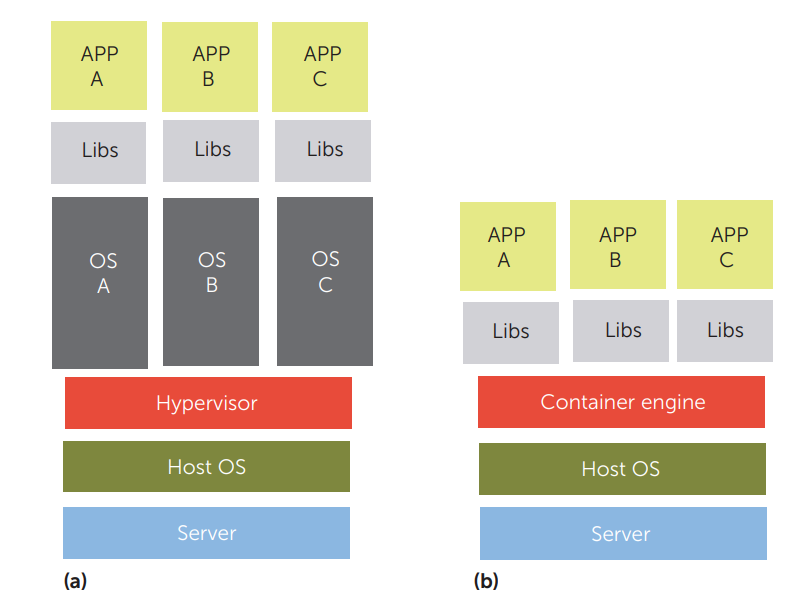
\includegraphics[width=0.8\textwidth]{images/bernstein-hypervisor-vs-container-deployment.png} 
  \caption{Comparison of (a) hypervisor and (b) container-based deployments (taken from source \cite{Bernstein2014})}
  \label{fig:compdeployment}
\end{figure}

Almost all mainstream players in the industry support and follow these \acrshort{oci} guidelines, effectively creating a strong standard in the industry with many benefits as a result. For example, outsourcing cloud management to public providers enables lower costs due to economy of scale, where the location cost of the servers is divided between all the users that run their applications on them. If you want to use these public providers you often only need to create and share your image. Changing providers for your deployment is also fairly easy thanks to this industry standardization, making for a competitive market. Furthermore, the portability of container images allows for quick deployments, compared to hypervisor deployments which require more manual configuration. 
\\[10pt]




% ===========================================
\section{Docker Engine} \label{sec:containerruntime}
Once an \acrshort{oci} standard image is created for an application and is stored in a registry it still needs to be deployed as a container. We previously talked about cloud providers, but even they need a way to turn the image into a running container. This is where container engines such as Docker Engine come into play \cite{dockerengine}. Container engines are the bridge between the end-user and the deployment of a container based on an image: they accept user requests and pull the images from the registry to run the container based on the metadata in the image. It also offers an API so the engine can be called by a higher abstraction layer such as \acrshort{k8s} (see \autoref{sec:kubernetes}). 
\\[10pt]

Container engines such as Docker engine not only run containers, but also manage dependencies and allow multiple containers to run on the same \acrshort{os} by using virtualization while keeping different applications separated for security reasons \cite{cnwiki}. \autoref{fig:deployment} shows an example of the usage of Docker Engine for the deployment of 4 containers that together provide 2 different services (S1 and S2). The engine itself only installs the required binaries and libraries for the containers as described in the image, and shares these between all the containers requiring them. This saves on resources and improves booting speed since binaries and libraries only need to be loaded once.
\\[10pt]

\begin{figure}[htbp]
  \centering
  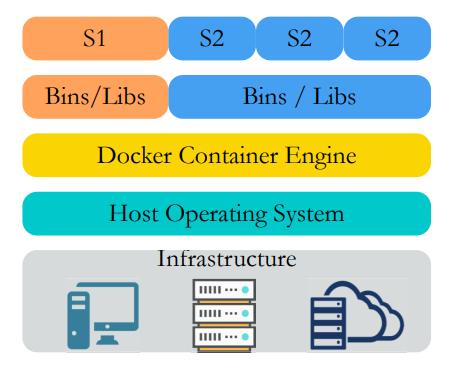
\includegraphics[width=0.4\textwidth]{images/docker-containers.png} 
  \caption{a container deployment using Docker Engine (taken from source \cite{resman})}
  \label{fig:deployment}
\end{figure}

When looking at the inner workings of Docker Engine we see that it is an open-source project build upon Moby\cite{moby}. Moby is a framework that consists of multiple plug-and-play components that enable you to manage images, configuration and secrets while providing networking and provisioning to your container, as seen in \autoref{fig:moby}. Docker engine thus offers some extra functionality for managing a container thanks to the Moby framework, but this does not yet explain how the image is run as a container, which brings us to container runtimes.
\\[10pt]

\begin{figure}[htbp]
  \centering
  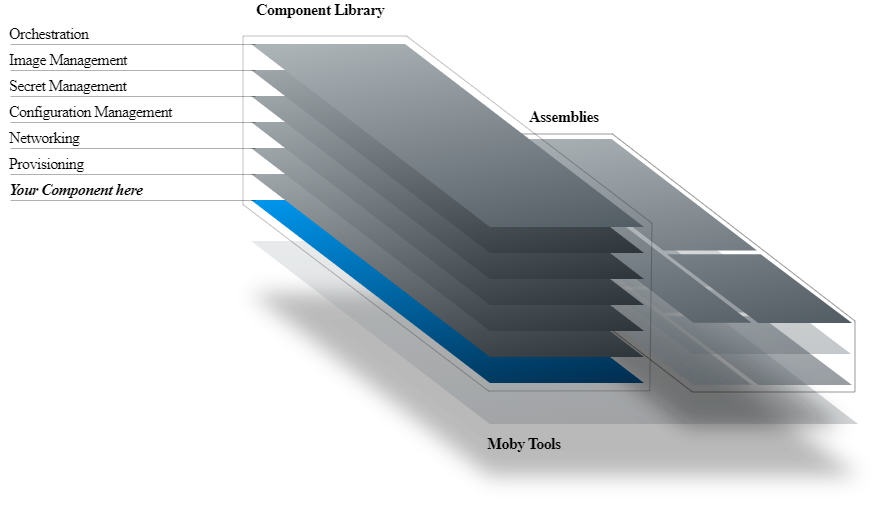
\includegraphics[width=0.8\textwidth]{images/moby.png} 
  \caption{Moby framework (taken from source \cite{moby})}
  \label{fig:moby}
\end{figure}

 Container runtimes manage the life-cycle of containers and serve as the bridge between the host system and the container \cite{containerterminology},\cite{contruntime}. when a container runtime is requested to run a container it will first pull the correct image from its image repository and will then ready the host system based on the metadata included in that image. This includes giving the container network attachments and storage if required. Afterwards, it will communicate with the kernel to start the container. container runtimes such as containerD \cite{containerd}, CRI-O \cite{crio} and Mirantis \cite{mirantis} adhere to \acrshort{oci}'s runtime specifications which means they are interchangeable. Our container engine, Docker Engine, is designed specifically with containerd under the hood.
\\[10pt]

When more functionality is required than Docker Engine can offer such as load balancing, integration with Docker Compose or image vulnerability scanning, then we need to look at container orchestration tools. In this thesis, we will be using \acrshort{k8s}, which will be described in the next section.
\\[10pt]



% =========================================
\section{Kubernetes}\label{sec:kubernetes}

Even though Docker Engine can easily deploy multiple containers, managing all of them can become challenging very quickly, especially as the size of your container cluster scales up to hundreds or thousands of containers. Issues such as container crashes, loss of network connectivity, running out of resources and many more can arise and need to be dealt with correctly. To help solve these challenges container orchestration tools were introduced such as Docker Swarm \cite{dockerswarm}, Apache Mesos \cite{apachemesos}, and the current industry standard \acrshort{k8s} \cite{resman} \cite{CNCFSurvey}. This thesis will research and utilise \acrshort{k8s}.
\\[10pt]

\acrfull{k8s} is an open-source platform that automates container orchestration whether it is for one, hundreds, or even thousands of containers and is supported by most major public cloud providers such as \acrfull{aws} \cite{aws}, Microsoft Azure \cite{azure} and \acrfull{gcp} \cite{gcp}. \acrshort{k8s} automates functionalities such as scaling, deployment, storage, rollbacks, load balancing, secret management and many more, all of which can be configured using specifications created by a cluster manager in YAML or JSON format. To have a better understanding of \acrshort{k8s} \autoref{fig:kubernetes} shows an overview of K8s components, where they are typically deployed and how they communicate with each other in a cluster. In the rest of this section, we will describe the \acrshort{k8s} components and concepts in the figure that are important for this thesis. 
\\[10pt]
\begin{figure}[htbp]
  \centering
  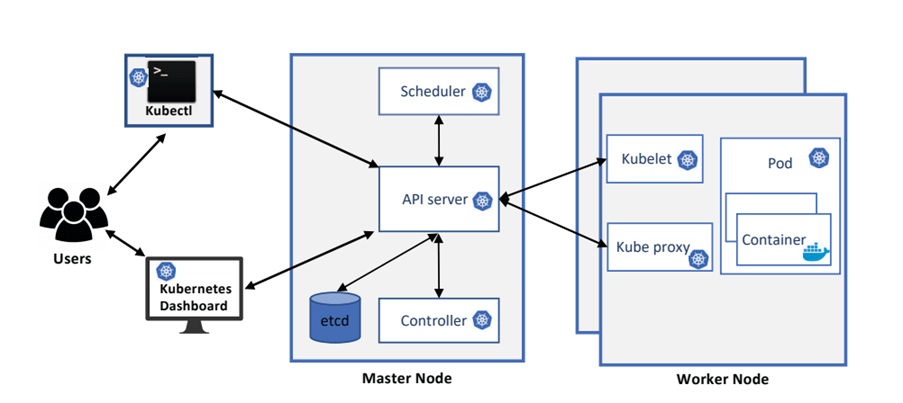
\includegraphics[width=0.8\textwidth]{images/kubernetes-structure.png} 
  \caption{a brief overview of \acrshort{k8s} (taken from source \cite{IslamShamim2020a})}
  \label{fig:kubernetes}
\end{figure}

\textbf{Node:} \label{comp:node} Nodes are the biggest component in a \acrshort{k8s} cluster and have two variations which are not mutually exclusive: worker and master nodes. They are machines, either virtual or physical, on which containerized applications run. Worker nodes host \hyperref[comp:pod]{pod(s)}, a \hyperref[comp:kubelet]{kubelet service} and a kube-proxy service. Master nodes on the other hand are part of the control plane and are responsible for managing the worker nodes. They host components such as the controller, scheduler, \hyperref[comp:apiserver]{API server} and etcd storage. These control plane components can be spread across multiple master nodes to provide fault tolerance. Each cluster needs at least one node to operate correctly but can easily scale up to thousands.  \cite{node}
\\[10pt]

\textbf{Pod:} \label{comp:pod} A pod is the smallest deployable computational component in a \acrshort{k8s} cluster, runs on a \hyperref[comp:node]{node}, and houses one or more containers that are tightly coupled. A pod remembers through its specification file how to run the container(s) it is responsible for and shares storage and network resources between them. If containers are tightly coupled they can run on a single pod to have unrestricted communication and shared resources, but this introduces some security concerns such as the possibility of malware spreading between those containers. Duplicates of containers can be deployed on separate pods to increase an application's workload (horizontal scaling). To redirect requests to an application without any notable difference for the end-user the load-balancer is introduced. It will automatically redirect requests to the application with the least current tasks to ensure optimal spreading of end-users. Alternatively to horizontal scaling the available resources for a pod can be increased (vertical scaling) to scale workload capabilities. \autoref{fig:pod} shows an example of a pod specification in the form of a YAML file. \cite{pod}
\\[10pt]

\begin{figure}[htbp]
  \centering
  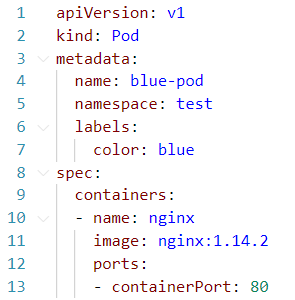
\includegraphics[width=0.5\textwidth]{images/pod.png} 
  \caption{an example pod specification}
  \label{fig:pod}
\end{figure}

\textbf{Kubelet:} \label{comp:kubelet} Each node in a cluster runs its kubelet service component. The kubelet manages all the \hyperref[comp:pod]{pods} on the same \hyperref[comp:node]{node} by deploying, monitoring and deleting them. The kubelet knows how to deploy these pods thanks to the PodSpec YAML or JSON file it receives from the \hyperref[comp:apiserver]{API server} in the control plane. By using the kubelet \acrshort{k8s} can ensure \hyperref[comp:pod]{pod} crashes get noticed and handled according to specifications. \cite{kubelet}
\\[10pt]

\textbf{API server:} \label{comp:apiserver} The \acrshort{k8s} API Server offers REST operations through which users can interact with the cluster. It takes user inputs from the command line interface Kubectl or a \acrshort{k8s} dashboard and communicates the necessary changes to the other components. It also validates requests and configures the data that passes through it. Libraries have been built on top of the REST operations to facilitate new ways to interact with the API server, and for this thesis, we shall be using the python \acrshort{k8s} library as the main method of communication with the cluster \cite{pythonk8s} \cite{kubeapiserver}.
\\[10pt]


\textbf{Namespace:} \label{comp:namespace} A namespace is a mechanism to separate groups of resources in a \acrshort{k8s} cluster. Within a namespace each resource must have a unique name, although equal names can exist in different namespaces. objects that are used cluster-wide, like a \hyperref[comp:node]{node} for example, do not allow the specification of a namespace. An example usage for a namespace would be the separation of different tenants according to their subscription plan on the cluster's resources \cite{namespace} \cite{feasability}.
\\[10pt]


\textbf{Labels:} \label{comp:label} Labels are key/value pairs which allow \acrshort{np}s to select pods. Multiple labels can be applied to a single object, much like a \acrfull{abac} system where attributes are linked to object \cite{abac}. Important to note is that for each object there can be no duplicate keys. e.g. applying \textit{role: database} and \textit{role: application} to a single object is not allowed and will result in errors. In the previously mentioned \autoref{fig:pod} we can see an example of a \acrshort{k8s} \hyperref[comp:pod]{pod} that has the label \textit{color: blue} attached to it. 
\\[5pt]

To retrieve all objects based on labels the use of label selectors is required.  If multiple label requirements are specified in a label selector then the found objects will have to match with not one but all of these requirements. Furthermore, there is a difference between equality-based requirements and set-based requirements. When using the first matching objects must satisfy the (non)-equality with a specific label, e.g. it must (not) have the label \textit{role: db}. The set-based requirement on the other hand offers three choices to be used with a set of values: \textit{in}, \textit{notin} and \textit{exists}. An example of a set-based requirement would be \textit{role in (database, application)} where either \textit{role: database} or \textit{role: application} would fulfil the requirement. \autoref{fig:np} shows an example of equality-based requirements in a network policy. \cite{labels}
\\[10pt]

\begin{figure}[htbp]
  \centering
  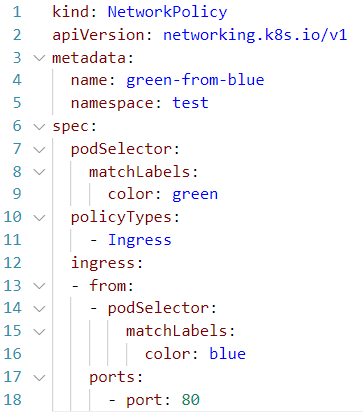
\includegraphics[width=0.5\textwidth]{images/np.png} 
  \caption{an example \acrshort{np} specification}
  \label{fig:np}
\end{figure}


\textbf{Network policy:} \label{comp:networkpolicy} A \acrfull{np} is used to control network traffic on the IP address or port level. \acrshort{np}s are applied only to pods, but can use different types of selectors: a namespace selector will just target all pods in the defined namespace, an ipBlock selector targets pods based on a match in IP, and lastly pod selectors target based on labels. This last option will only look at pods with matching labels in the same namespace in which the \acrshort{np} is deployed. In this thesis, we only focus on pod selectors with labels and work in a single namespace.
\\[10pt]
To describe the general build of a \acrshort{np} we will look back at \autoref{fig:np}. We can see that the \acrshort{np} is in the namespace \textit{test} and that it selects pods that have the label \textit{color: green}. This \acrshort{np} will thus only apply to pods in the namespace test with the same label. There are two types of policies: Ingress policies that define from which pod communication is allowed and egress policies that define to which pod communication is allowed. Thus the example \acrshort{np} in \autoref{fig:np} specifies that all pods with the label \textit{color: green} in the namespace test are allowed to accept communication from all pods with the label \textit{color: blue} in that same namespace.
\\[10pt]


Important to note is that this does not mean pods with the label \textit{color: blue} are allowed to send messages to pods with the label \textit{color: green} yet. For this, we need a correctly defined egress rule as well. In practice, at least two \acrshort{np}s are required for pods to communicate. \cite{k8snp}



% =========================================
\section{Kano}\label{sec:kano}
Although \acrshort{np}s offer extra security for a \acrshort{k8s} cluster it also has its drawbacks. They need to be closely managed to ensure no contradictions are specified and that containers can connect to another container they rely upon. To combat these difficulties Kano was introduced by researchers at the Tsinghua University in Bejing.
\\[10pt]
Kano is a container \acrshort{np} verification tool presented in 2020 that, to quote the authors, solves the following problem: "In a container network, do the network
policies violate the network constraints?" \cite{kano}. It does so by creating a matrix representing the container connections based on the existing network policies. Once this matrix is created it is leveraged to find underlying issues such as redundant \acrshort{np}s or an isolated container and those issues are reported to the user. We will continue to explain Kano in more detail since the solution algorithm of this thesis builds directly on some of Kano's concepts.
\\[10pt]

\textbf{Kano Reachabilitymatrix:} \label{kano:matrix} Kano starts by modelling a container network as a bipartite graph where the vertices are containers with 2 sets of edges \textit{E1} and \textit{E2}: ingress and egress \acrshort{np}s respectively. \autoref{fig:kano-bipartite-graphs} depicts this, but in 2 bipartite graphs instead of one to easily separate between the ingress and egress sets. The intersection of these sets  ($\textit{E1} \cap \textit{E2}$) represents connections between pods allowed by both an ingress and an egress rule. To save storage space and to allow quicker computations Kano does not save the container network as a bipartite graph, but as a matrix with bit arrays as rows, which we will call the kanomatrix or reachability matrix from now on. The kanomatrix is a square matrix of size \(kxk\) where \(k\ =\ amount\  of\  containers\  in\  the\  cluster\). A 1 in position [i][j] means that the container with index [i] can communicate towards the pod with index [j] respectively. \autoref{fig:kano-reach-matrix} shows the ingress and egress matrix that correspond to the bipartite graphs in \autoref{fig:kano-bipartite-graphs}, as well as the final kanomatrix which is equal to the intersection of the two matrices, achieved by using the bitwise AND operation between the matrices' bit arrays.
\\[10pt]

\textbf{Prefiltration algorithm:} \label{kano:prefiltration} In a container cluster changes happen frequently and therefore the reachability matrix need to be generated often. A naive solution to generate the reachability matrix would be to iterate over all policies and match them with containers with corresponding labels. This solution is not scalable to execute for every change since the time complexity would be $O(mn)$ with $m\ =\ number\ of\ policies$ and $n\ =\ number\ of\ containers$. To counter this Kano introduced a prefiltration algorithm based on bit arrays. The algorithm starts by creating a hashmap, where each key is a label that is applied to at least one container, and the values are bit arrays with a length equal to the number of containers in the cluster. In such a bit array the position of a set bit represents that the container with its index equal to that position has the corresponding label key applied. This is seen in \autoref{fig:kano-cont-prefiltration}.
\\[10pt] 

\begin{figure}
\centering
    \begin{minipage}[b]{0.8\linewidth}
        \centering
        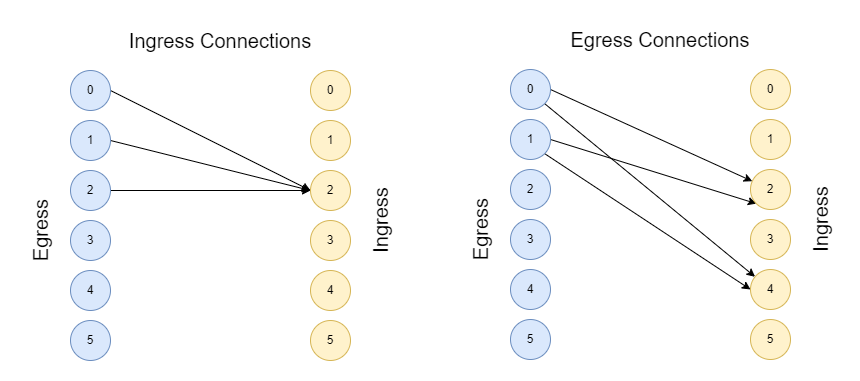
\includegraphics[width=0.8\textwidth]{images/kano-combined-connections-graph.png} 
        \caption{Bipartite graphs for Kano matrix generation} 
        \label{fig:kano-bipartite-graphs}
    \end{minipage}
    \begin{minipage}[b]{0.8\linewidth}
         \centering
          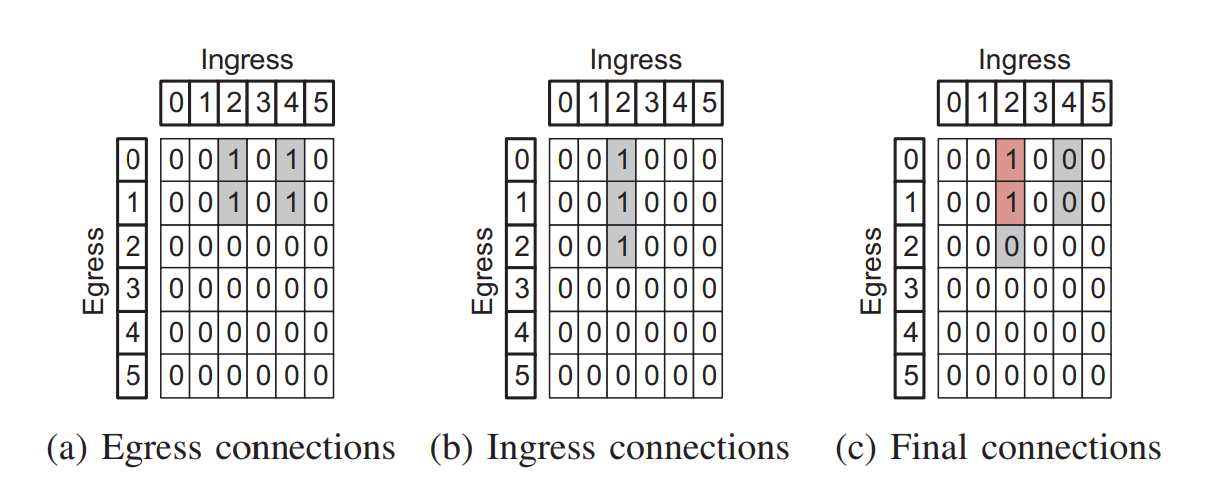
\includegraphics[width=0.8\textwidth]{images/kano-matrix-generation.png} 
          \caption{Container network reachability matrix model (taken from source \cite{kano})} 
          \label{fig:kano-reach-matrix}
    \end{minipage}
      
\end{figure}

When searching the containers to which a \acrshort{np} applies we retrieve the bit arrays corresponding to the selector labels of a policy in the hashmap. By applying a bitwise AND opperation to these bit arrays we get a bit array with bits set for each container that matches all labels from the policy. This is illustrated in \autoref{fig:kano-pol-prefiltration}. The time complexity of creating the hashmap based on the containers is $O(m)$, while the lookup for a policy is $O(1)$, which is a drastic improvement on the naive solution.
\\[10pt]

\begin{figure}[htbp]
  \centering
  \begin{minipage}[b]{0.45\linewidth}
    \centering
    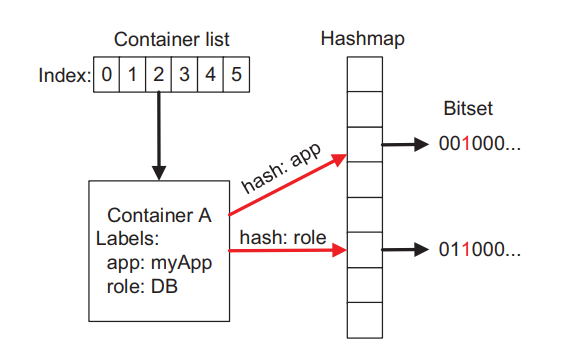
\includegraphics[width=\textwidth]{images/prefil_cont_labels.png}
    \caption{Prefiltration of container labels (taken from source \cite{kano})}
    \label{fig:kano-cont-prefiltration}
  \end{minipage}
  \quad % Add some horizontal space between the subfigures
  \begin{minipage}[b]{0.45\linewidth}
    \centering
    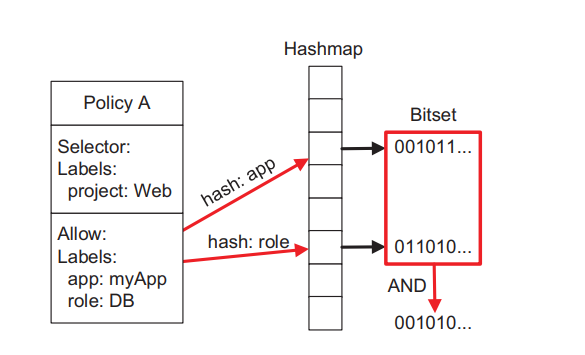
\includegraphics[width=\textwidth]{images/prefil_pols.png}
    \caption{Prefiltration of policies (taken from source \cite{kano})}
    \label{fig:kano-pol-prefiltration}
  \end{minipage}
\end{figure}

\textbf{Violation check:} \label{kano:violationcheck} Once the reachability is created with the prefiltration algorithm it can be used to verify some violations. The following descriptions are taken directly from the Kano paper \cite{kano}:
\begin{itemize}
    \renewcommand{\labelitemi}{\scriptsize$\blacksquare$}
    \item \textit{All reachable:} A container can be reached by all containers.
    \item \textit{All isolated:} A container cannot be reached by any container.
    \item \textit{User cross:} A container can reach another user’s container in the container network.
    \item \textit{Policy shadow:} The connections built by a policy are completely covered by another policy, then this policy may be redundant
    \item \textit{Policy conflict:} The connections built by a policy contradict the connections built by another.
\end{itemize}
Additionally, you can define your constraints with the use of declarative language, for example, to guarantee two containers can communicate. Since the violation checker will not be used in this thesis we will not go into detail about its implementation
\\[10pt]


% =========================================
\section{Calico}\label{sec:calico}

Pods, and by extension containers, in a \acrshort{k8s} cluster are not able to communicate with each other by default. Instead, you need to either explicitly create links between the pods or give each pod its unique IP address within the cluster. The latter option of two is called the \acrshort{k8s} network model, and to achieve it a \acrfull{cni} plugin is required. \cite{k8scni} \cite{k8snetworkmodel}. The \acrshort{cni} is a specification for writing plugins that should only be concerned with network connectivity of containers and deleting these as the container gets removed \cite{cni}. Many plugins based on the \acrshort{cni} project exist, such as Weave \cite{weave}, Cilium \cite{cilium} and Project Calico \cite{calico}.
\\[10pt]

There are some rules that \acrshort{k8s} set to which \acrshort{cni} plugins must adhere before being allowed into the ecosystem. First and foremost pods must be able to communicate with each other, independently of the node on which they are deployed without the necessity of \acrfull{nat}. Secondly, all \acrshort{k8s} components on a node such as the kubelet and kube-proxy must be able to communicate with all pods on that node. Together these 2 rules guarantee that \acrshort{cni} plugins do not hinder the working of the \acrshort{k8s} cluster, but still allow freedom for the addition of functionalities.
\\[10pt]

Calico has been chosen for this thesis to ensure ready-to-go communication between the containers for testing purposes. Calico offers specific optimisations for \acrshort{k8s} by using eBPF, a Linux kernel feature that allows you to run a \acrshort{vm} inside the kernel itself \cite{ebpf}. This means that Calico does not have to rely on the default iptables-based Linux standard for network routing and can improve latency and performance with its solutions. Calico also enforces the \acrshort{k8s} \acrshort{np}s and, although not used in this thesis, offers its own type of network security rules on top of the default \acrshort{k8s} ones if required. The last reason we choose Calico instead of one of the alternatives is the default support for VM networking with OpenStack, thanks to the Neutron ML2 plugin \cite{neutron}. 


% =========================================
\section{Openstack}\label{sec:openstack} To host our nodes in a \acrshort{k8s} cluster we have two options: Using physical devices or \acrlong{vm}s. The second option not only reduces overhead, but requires no extra physical hardware if your existing hardware has enough resources, and can thus be scaled easily according to the needs of the cluster. Just like physical machines \acrshort{vm}s need to be managed, and this is where virtual operating systems come into play, often synonymously called cloud operating systems due to cloud native computing becoming the standard \cite{CNCFSurvey}. Some examples of cloud operating systems are Google Chrome OS \cite{chromeos}, \acrshort{aws} \cite{aws} and OpenStack, which is our tool of choice for this thesis \cite{Openstack}.
\\[10pt]

OpenStack automates the management of computing and network resources for clusters of physical and virtual machines, which can be easily directed through the dashboard application or directly via the API. OpenStack has great modifiability by allowing cluster administrators to extend their cluster with the components of their choice with example categories such as hardware life-cycle, storage, orchestration and application life-cycle. A \acrshort{vm} deployed with OpenStack is called an instance, and in this thesis, OpenStack is used to deploy instances that host our \acrshort{k8s} nodes. OpenStack also has network security solutions to manage connections between instances, which we describe more in-depth in the following paragraphs.
\\[10pt]

\textbf{Security Groups}\label{sec:securitygroups} Security Groups are a way to group network security rules together to be easily applied to instances within the OpenStack cluster. They are identified by their name, which must be unique within the cluster and can carry a description to describe their intended usage. Every instance has the $default$ security group applied if no custom are linked. This default security group denies all incoming traffic and allows only outgoing traffic to your instance. A limit can be imposed on the maximum rules per security group and on the maximum defined security groups in the cluster by the security group's quota. \cite{sg} \cite{sgquotas}
\\[10pt]

\textbf{Security Group Rules}\label{sec:securitygrouprules} Security group rules use IP filters to allow or block communication from certain IPs. These rules also specify a protocol for which they are applied, with the choices being TCP, UDP or ICMP. When wanting to target multiple protocols multiple security group rules are needed. The IP or IP range on which the rule applies must be specified in CIDR notation and a port range can be included as well. Alternatively to selecting IPs, another security group can be targeted instead, with the advantage that instances can be added or removed from security groups without the need for revision of the security group rules. \autoref{fig:sgrule} shows a security group with the name $open$ that holds two security group rules, one for UDP and one for TCP but both selecting all possible IPs and ports (65535 being the highest value of an unsigned 16-bit integer and thus the highest possible port value). \cite{sgrule}
\\[10pt]

\begin{figure}[htbp]
  \centering
  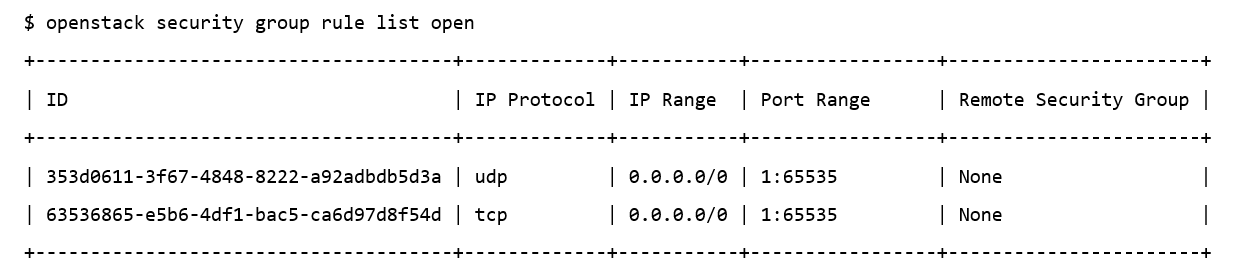
\includegraphics[width=\textwidth]{images/sgrule example.png} 
  \caption{Security group rule example (taken from source \cite{sg}}
  \label{fig:sgrule}
\end{figure}

\cleardoublepage
